\documentclass[conference]{IEEEtran}
\ifCLASSINFOpdf 
\else
\fi
\hyphenation{op-tical net-works semi-conduc-tor}
\usepackage{amsmath}
\usepackage{graphicx}
\usepackage{float}
\usepackage{subfig}

\begin{document}

\title{ENPM673 - Perception for Autonomous Robots\\Project 1}

\author{\IEEEauthorblockN{Saurabh Palande (UID: 118133959)}
\IEEEauthorblockA{Masters in Robotics Engineering\\
University of Maryland College Park\\
Email: spalande@umd.edu\\
}}


\maketitle

% As a general rule, do not put math, special symbols or citations
% in the abstract
\begin{abstract}
This project focuses on detecting a custom AR Tag (a form of fiducial marker),that is used for obtaining a point of reference in the real world, such as in augmented reality applications. There are two aspects to using an AR Tag, namely detection and tracking, both of which are implemented in this project. The detection stage involves finding the AR Tag from a given image sequence while the tracking stage involve keeping the tag in “view” throughout the sequence and performing image processing operations based on the tag’s orientation and position.
\end{abstract}

\IEEEpeerreviewmaketitle



\section{Problem 1 - Detection}
\subsection{Problem 1A}
% no \IEEEPARstart
In this part, the AR tag is detected using the Fast Fourier Transform(FFT). When we apply FFT to an image, it converts the image from spatial domain to frequency domain.Low frequencies are situated towards the center of the image and high frequencies scattered around.\\
Steps to detect AR tag using FFT:-
\subsubsection{Convert to grayscale and blur the image}
First step is to convert the image to gray scale and then blur it by using a low-pass filter to reduce the amount of noise and detail in an image. By blurring an image prior to applying techniques such as edge detection reduces the amount of high-frequency content, such as noise and edges.
\subsubsection{Generating mask}
The next step is to generate a mask to remove the background and the white paper surrounding the AR tag. To generate the mask, first the corners of the white paper are found. Then a mask is created using cv2.fillPolly with these 4 corner points where the region inside these 4 points is black and the background is white. The black region is dilated so that it entirely covers the region inside the white paper. The input image and the mask generated is shown in Figure 1.
\begin{figure}[H]
  \centering
  \subfloat[Input Image]{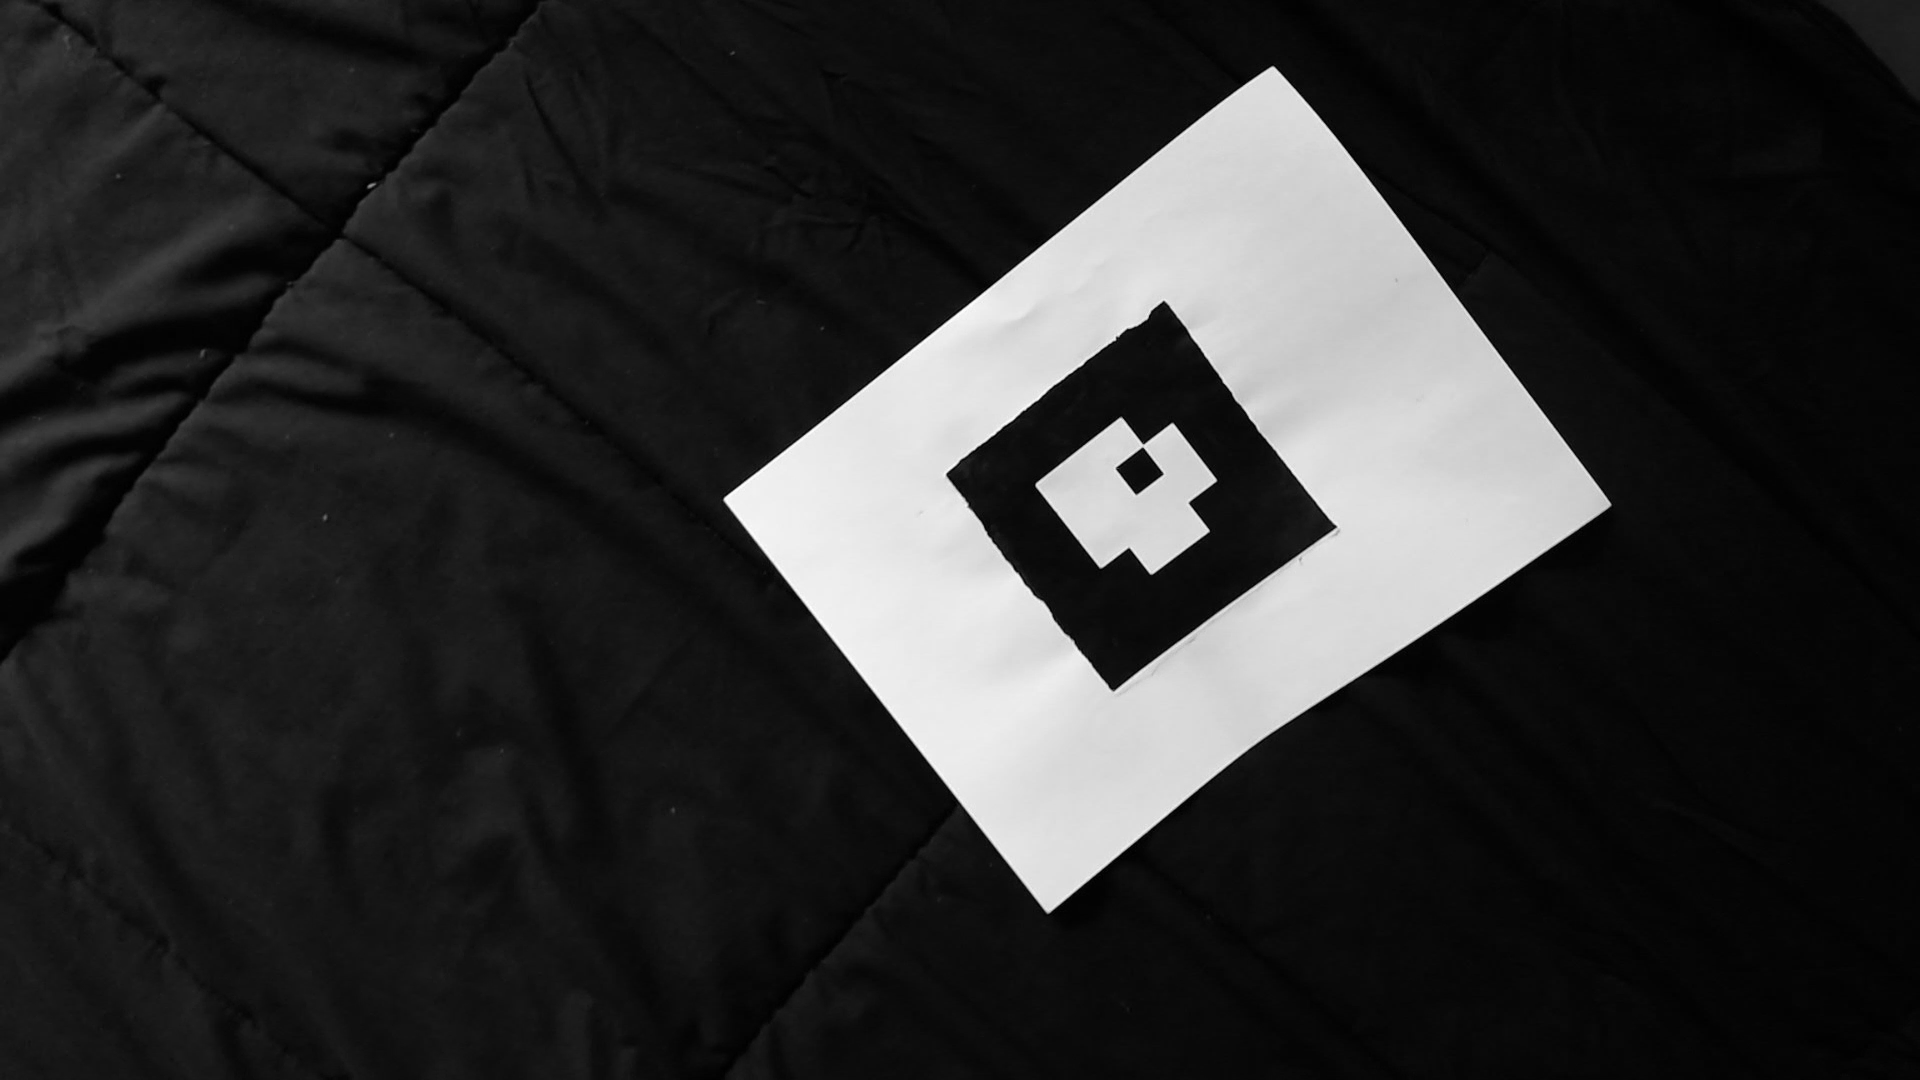
\includegraphics[scale = 0.062]{./Images/ARTag_frame.png}\label{fig:f1}}
  \hspace{.15cm}%
  \subfloat[Mask]{
\includegraphics[scale = 0.062]{./Images/mask.png}\label{fig:f2}}
  \caption{Input image and its corresponding mask}
\end{figure}

\subsubsection{Adding the mask to the thresholded and blurred image}
The mask is then added to the thresholded and the blurred image. After adding, the black background in the original image becomes white and the region inside the white paper remains the same. So now we have an image where only the AR tag is visible on a white background. The masked image is shown in Figure 2.
\begin{figure}[H]

\includegraphics[scale=0.08]{./Images/masked_image.png}
\centering
\caption{Masked image}
\end{figure}
\subsubsection{Applying FFT and inverse FFT}
FFT is applied to the masked image to convert it from spatial domain to frequency domain to find the edges. After taking a FFT of the masked a High Pass Filter (a mask array which has a circle of zeros in the center and rest all ones) is applied to this FFT transformed image. This filter would in turn block all low frequencies and only allow high frequencies to go through. Finally, inverse FFT is applied on this filter applied image to see the distinct edges of the AR tag. The FFT of the image and the FFT after HPF is shown in Figure 3. The final output is shown in Figure 4.
\begin{figure}[H]
  \centering
  \subfloat[FFT image]{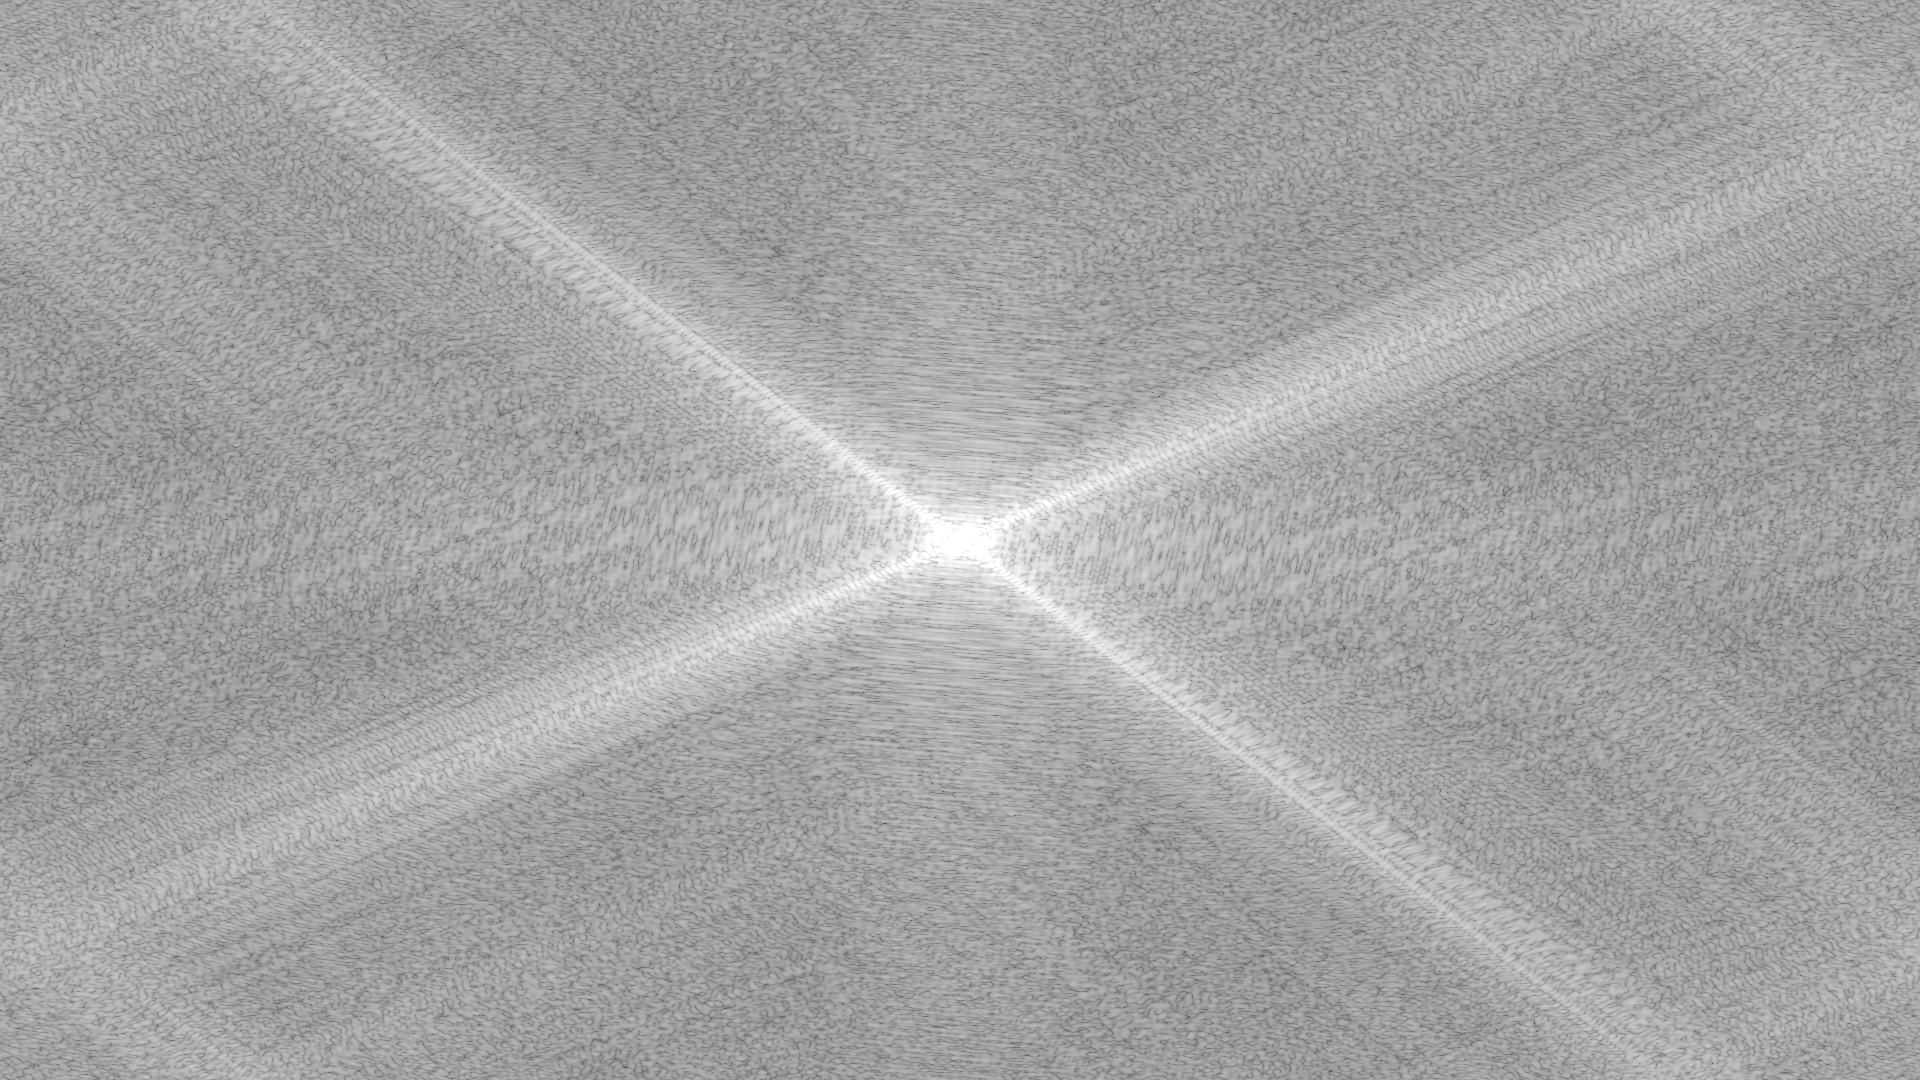
\includegraphics[scale = 0.058]{./Images/fft.png}\label{fig:f1}}
  \hspace{.15cm}%
  \subfloat[FFT after HPF]{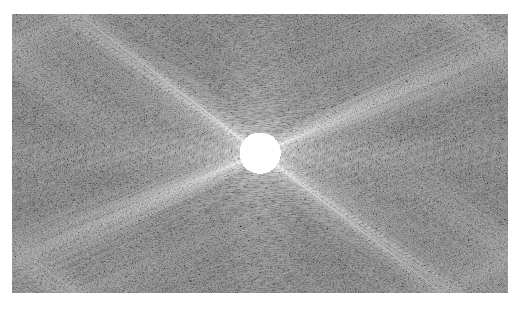
\includegraphics[scale = 0.3]{./Images/HPF_filtered.png}\label{fig:f2}}
  \caption{FFT and FFT after high pass filtering}
\end{figure}
\begin{figure}[H]
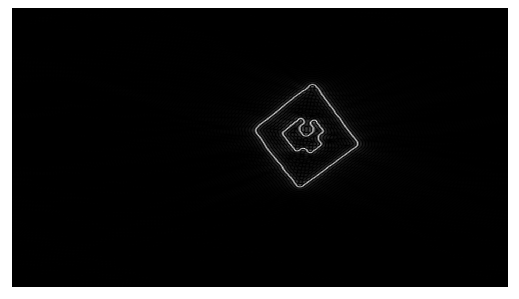
\includegraphics[scale=0.45]{./Images/ARTag_edges.png}
\centering
\caption{Detected AR tag using FFT}
\end{figure}
\subsection{Problem 1B}
To decode the custom AR tag the following steps are followed.
\subsubsection{Detect the tag}
The first step is to detect the tag in the video frames. To detect the tag the steps mentioned in Setion A.1, section A.2 and section A.3 are followed. Once we have the masked image, the 4 corner points are of the AR tag are extracted using the minimum and maximum condition on the x and y indices of the black pixel. 
\subsubsection{Warp the tag}
Next step is to warp the tag so that it can be decoded. Once the 4 corners of the tag are found, they are sorted in the order $[top-left, top-right, bottom-right, bottom-left]$. After that, homography between these 4 points and a planar set of reference points is computed using the below mentioned steps.
Each pair of corresponding points gives us two linearly-independent equations;
eight linearly-independent equations are formed by using four pairs of corresponding points. A homography has eight degrees of freedom, and is therefore fully determined by at least four correspondences. The homography matrix can be solved by writing these eight equations in matrix form. The A matrix is 
\\

\begin{bmatrix}
{x_1}^w & {y_1}^w & 1 & 0 & 0 & 0 & $-${x_1}^c {x_1}^w & $-${x_1}^c {y_1}^w & $-${x_1}^c\\
0 & 0 & 0 & {x_1}^w & {y_1}^w & 1 & $-${y_1}^c {x_1}^w & $-${y_1}^c {y_1}^w & $-${y_1}^c\\
: & : & :& :& : &:&:&:& :\\
{x_4}^w & {y_4}^w & 1 & 0 & 0 & 0 & $-${x_4}^c {x_4}^w & $-${x_4}^c {y_4}^w & $-${x_4}^c\\
0 & 0 & 0 & {x_4}^w & {y_4}^w & 1 & $-${y_4}^c {x_4}^w & $-${y_4}^c {y_4}^w & $-${y_4}^c\\
\end{bmatrix}\\

The h matrix is\\

\begin{center}

\begin{bmatrix}

h_{11}\\
h_{12}\\
h_{13}\\
h_{21}\\
h_{22}\\
h_{23}\\
h_{31}\\
h_{32}\\
h_{33}\\
\end{bmatrix}
\end{center}\\

We can calculate the homography using the equation 1. The solution to this equation can be found out using SVD.Decompose matrix A via SVD: [ U, S, V ].The elements of homography, h, are obtained from the last column of V. Since $h_{33}$ should be 1, V should be normalized using $v_{99}$ :
\begin{equation}
Ah = 0_{8*1}
\end{equation}
After computing the homography matrix inverse warping is done to obtain the AR tag for decoding.
\subsubsection{Decode the tag}
The following are the steps to decode the orientation and the ID of the AR tag:
\begin{enumerate}
\item The tag can be decomposed into an 8 x 8 grid of squares, which includes a
adding of 2 squares width (outer black cells in the image) along the borders.
This allows easy detection of the tag when placed on any contrasting
background.
\item After the borders are cropped, take the median of the values in the 4 corner grids and check for a high value. Only one corner of the AR tag should have a high value. If more than one corner has a high value it is discarded
\item The tag is rotated till the bottom right corner value become high and the angle by which it is rotated becomes the orientation of the AR tag.
\item Lastly, the inner-most 2 x 2 grid (i.e. after removing the padding and the
orientation grids) encodes the binary representation of the tag’s ID,
which is ordered in the clockwise direction from least significant bit to
most significant. So, the top-left square is the least significant bit, and
the bottom-left square is the most significant bit.
\end{enumerate}
The four corners of the decoded AR tag and the orientation and the Tag ID for one of the frames is shown in Figure 5.
The entire video of the detected and decoded AR tag can be found here (LINK)
\begin{figure}[H]
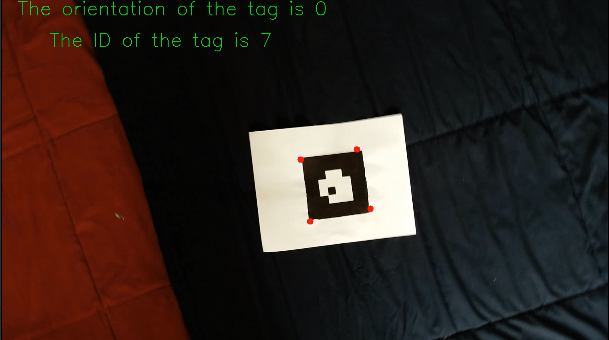
\includegraphics[scale=0.4]{./Images/ar_tag_corner.png}
\centering
\caption{Detected and decoded AR tag}
\end{figure}
\begin{thebibliography}{1}

\section{Problem 2}
\subsubsection{Problem 2A}
In this section a template image (Testudo) is warped on the AR tag using the Homography matrix. Once the 4 corners of the AR tag are detected using the steps mentioned in the above section, we compute the homography between the AR tag corners and the testudo image corners (the image is resized to (320,320)).
Once the homography matrix is computed, the testudo is warped on the AR tag by using inverse warping. Based on the indices or pixel locations of the template image we calculate the pixels to be replaced in the original image by multiplying the template image indices by the homography matrix. Then the template image pixels are copied into the corresponding pixels of the original image as shown in Figure 6.
\begin{figure}[H]
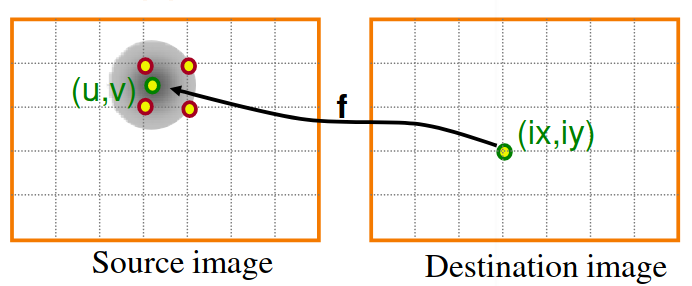
\includegraphics[scale=0.4]{./Images/inverse_warp.png}
\centering
\caption{Inverse Warping}
\end{figure}
\begin{thebibliography}{1}
\bibitem{filters}

\end{thebibliography}




% that's all folks
\end{document}


